\section{Concurrent updates for Linux kernel}

\subsection{Case study:reverse mapping}

%$$$$$$$$$$$$$$$$$$$$$$$$$$$$$$$$$$$$$$$$$$$$$$$$$$$$$$$$$$$$$$$$$$$$$$$$$$$$$$$$
%Paragraph 1: Linux의 reverse mapping에 대한 자세한 설명 
%$$$$$$$$$$$$$$$$$$$$$$$$$$$$$$$$$$$$$$$$$$$$$$$$$$$$$$$$$$$$$$$$$$$$$$$$$$$$$$$$

\ifkor
리눅스 커널의 프로세스간 공유자원 중 하나인 reverse page mapping(rmap)은 fork, exit, mmap이 수행될 때
update가 많이 발생하는 data structure이다.
Linux's reverse mapping reads walked through each process’s pages mappings and
selected pages to unmap when it swaps a pyhsical page out to disk, migrates
other cpu, or turncates a file.
After all a page’s mappings were removed could it be selected for
pageout~\cite{OBJMAPOLS}.
Rmap의 anonymous page와 file page의 관리는 최근 interval trees로 되어 있으며, 이것은 reverse page
성능 향상으로 위해 지속적으로 최적화가 ~\cite{CorbetLWNRMAP}~\cite{CorbetLWNANON} 이루어지고 있다. 
\else
%리눅스 커널의 프로세스간 공유자원 중 하나인 reverse page mapping(rmap)은 fork, exit, mmap이 수행될 때
%update가 많이 사용하는 data structure이다.
The reverse page mapping(rmap) a kernel memory management mechanism, and
consists of anonymous rmap and the file rmap.
These two rmap maintains virtual address (VMAs) in order to translate physical
addresses to virtual addresse[], and are a shared global resource.
These global resource of rmap are managed by using interval tree, and any
processes can update the one.
To protect the shared interval tree, the Linux use a semaphore.
This update operations such as tree's insert and remove operation are invoked by
fork, exit and mmap, so simultaneous creation of many processes causes
bottlenect becasue not only the update can not run in palarrel but also update's
lock can cache invalidation traffic.
On the contrary, the rmap reads walked through each process’s pages
mappings and selected pages to unmap when it swaps a pyhsical page out to disk, migrates
other cpu, or turncates a file.
After all a page’s mappings were removed could it be selected for
pageout~\cite{OBJMAPOLS}.
%Rmap의 anonymous page와 file page의 관리는 최근 interval trees로 되어 있으며, 이것은 reverse
% page 성능 향상으로 위해 지속적으로 최적화가 ~\cite{CorbetLWNRMAP}~\cite{CorbetLWNANON} 이루어지고 있다. 
This section show how to apply LDU to Linux to solve these bottlent, and it
deals with more practical contents.
\fi

\ifkor
리눅스는 rmap의 interval tree를 보호하기 위해 rw semapore를 사용한다. 
따라서, 프로세스들이 fork, exit, mmap를 simultaneosly 수행하면 interval tree를 보호하는
read-write semapore 때문에 scalability가 떨어진다.
anonymous page를 위한 rmap과 file mapped page을 위한 rmap 모두 문제가 있다.
이번 장은 이러한 문제를 해결하기 위해, 어떻게 LDU를 리눅스의 rmap에 적용했는지에대한 내용을 설명하며, 보다 practial한 내용을
다룬다.
\else

\fi
%The Linux rmap implementation can become a bottleneck when many processes
% simultaneously try to map the same file.
%For exemaple, simultaneous creation of many processes is likely to cause
% contention for the lock protecting the interval tree of the libc library,

%Objmap
%rmap is a mechanism for translating physical addresses to user virtual
% addresse.
%commonly called reverse mapping, or rmap. 
%This meant it was not possible for the memory management subsystem to point to
% a physical page and remove all its mappings. 
%There was a mechanism that walked through each process’s mappings and selected
%pages to unmap.
%Only after all a page’s mappings were removed could it be selected for pageout

%Many in the memory management community considered this very inefficient.
%Page aging and removal could be made much more efficient if the page could be
%directly unmapped when it was ready to be removed.
%Some form of rmap was clearly needed for this to work.

%Oplog
%Linux's reverse map(ramp) records, for each physical page, all page table
% entries that map that page.
%Linux reads these reverse mappings when it truncates a file or swaps a physical
% page out to disk, in order to find(and then delete) all page table entries
% that refer to the deleted page(s).
%The fork(), exit(), and mmap() system calls update the rmap, but don't need to
% read it.
%The Linux designers have heavily optimized the rmap using interval
% trees[21, 22, 24].
%Each file has an associated interval tree protected by a lock.
%A file's interval tree maps intervals of the file to virtual address mappings.
%Each virrtual address mapping maps one or more pages from the file.
%The Linux rmap implementation can become a bottleneck when many processes
% simultaneously try to map the same file.
%For exemaple, simultaneous creation of many processes is likely to cause
% contention for the lock protecting the interval tree of the libc library,
% because creating a process entails creating virtual address mappings for libc
% and inserting the mappings into the libc ramp interval tree.


\subsection{anonymous mapping}


\begin{figure}[tb]
  \begin{center}
     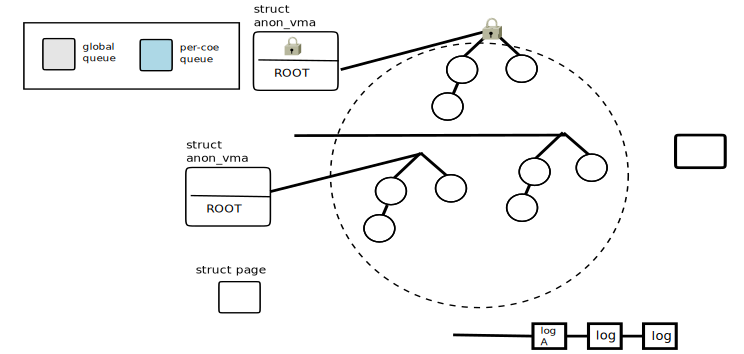
\includegraphics[width=0.5\textwidth,height=0.5\textheight,keepaspectratio]{fig/anon_vma}
  \end{center}
  \caption{An example of applying the \deferu to file reverse mapping. }
  \label{fig:deferu2}
\end{figure}

%$$$$$$$$$$$$$$$$$$$$$$$$$$$$$$$$$$$$$$$$$$$$$$$$$$$$$$$$$$$$$$$$$$$$$$$$$$$$$$$$
%Paragraph 1: linux의 anon vma의 공유된 구조에 대한 설명
%$$$$$$$$$$$$$$$$$$$$$$$$$$$$$$$$$$$$$$$$$$$$$$$$$$$$$$$$$$$$$$$$$$$$$$$$$$$$$$$$
\ifkor
Anonymous rmap의 공유데이터는 서로 상당히 복잡하게 연결되어 있다. 
그림 x-x는 이렇게 복잡하게 연결된 공유데이터를 보여준다.
fork가 수행되면 부모의 anon\_vma\_chain(avc)는 복사가 되며 해당 avc를 관리하는 새로운 anon\_vma가 생성된다. 
여기서 Anonymous rmap의 file rmap과 다른점은 자식에 해당하는 anon\_vma에 대한 tree operation을
수행할 때 사용되는 lock은 root가 가지고 있는 lock을 이용한다. 
따라서 자식이 많아지는 경우 root의 lock 때문에 심한 lock contention이 발생한다[].
\else
%fork가 수행되면 부모의 anon\_vma\_chain(avc)는 복사가 되며 해당 avc를 관리하는 새로운 anon\_vma가 생성된다. 
When a process spawns, the parent's anonymous vma chain(avc) are copyed to
child, and then the new anonymous vma indicating the child's avc is created.
%Anonymous rmap의 공유데이터는 서로 상당히 복잡하게 연결되어 있다. 
%그림 x-x는 이렇게 복잡하게 연결된 공유데이터를 보여준다.
Due to the fact that the continuous process spawns, it become more complex
anonymous ramp data structre.
That is, the anonymous ramp is one of the complex data structure in the Linux
kernel[].
Figure x-x shows this complex anonymous rmap data structure.
%여기서 Anonymous rmap은 자식에 해당하는 anon\_vma에 대한 tree operation을
%수행할 때 사용되는 lock은 root가 가지고 있는 lock을 이용한다. 
To prevent the udpate operations for the interval tree, the anonymous rmap
uses root lock, so when the that makes the Linux fork.
Therefore, when the child is increased, root lock makes lock contention
problem[].
\fi


%$$$$$$$$$$$$$$$$$$$$$$$$$$$$$$$$$$$$$$$$$$$$$$$$$$$$$$$$$$$$$$$$$$$$$$$$$$$$$$$$
%Paragraph 2: anon vma에 ldu 적용한 방법에 대한 설명 
%$$$$$$$$$$$$$$$$$$$$$$$$$$$$$$$$$$$$$$$$$$$$$$$$$$$$$$$$$$$$$$$$$$$$$$$$$$$$$$$$
\ifkor
이러한 lock contention을 제거하기 위해 LDU는 각각의 anon\_vma\_chain object에 대해서
mark 필드를 추가하여, update-side removing을 수행한다.
anonymous rmap역시 global queue를 사용한다면, lock을 root의 lock을 사용하기 때문에, log의 위치는 그림
x-x와 같이 root의 anon\_vma에 해당하는 object에 로그를 저장한다. 
만약 percore queue를 사용하면, percore에 위치에 root 포인터 정보와 함께 operation log를 저장한다.
\else

%이러한 lock contention을 제거하기 위해 LDU는 각각의 anon\_vma\_chain object에 대해서
%mark 필드를 추가하여, update-side removing을 수행한다.
In anonymous ramp, in order to eliminate the lock contention, LDU adds insert
and remove mark field in avc object for concurrent update, and it performs the
update-side removing logs.
%앞에서 설명한 봐와 같이, anonymous rmap는 root의 lock을 사용하기 때문에, 로그를 저장하는
%위치를 global queue를 사용한다면, x-x와 같이 root의 anon\_vma에 해당하는 object에 로그를 저장하고,
%per-core queu를 사용한다면 root 정보와 함께 log를 per-core 메모리에 저장한다.
Understanding the log's position of queue header in anonymous rmap is important.
As noted earlier, since anonymous rmap locks using the root lock, LDU global
queue logs in the position of the root data structure, and the per-core queue
also logs in the per-core queue with root information.
\fi


\subsection{file mapping}

%$$$$$$$$$$$$$$$$$$$$$$$$$$$$$$$$$$$$$$$$$$$$$$$$$$$$$$$$$$$$$$$$$$$$$$$$$$$$$$$$
%Paragraph 1: linux의 file mapped page reverse mapping의 구조에 대한 설명
%$$$$$$$$$$$$$$$$$$$$$$$$$$$$$$$$$$$$$$$$$$$$$$$$$$$$$$$$$$$$$$$$$$$$$$$$$$$$$$$$
\ifkor
file을 위한 rmap의 구조는 그림 x과 같다. 
reverse page map을 위한 page는 inode가 가지고 있는 address\_space를 가리키며, 이것은
vm\_area\_struct(vma)을, containg the virtual address of the mapping, interval
tree를 이용하여 관리한다. 이것은 fork가 되면 부모의 address\_space의 interval tree에 추가된다.
Tree를 보호하기 위한 lock은 프로세스마다 공유하는 데이터인 address\_space의 lock을 사용하여
보호되며, anonymous ramp의 lock보다 contention이 덜 발생 하지만, file ramp역시 fork, exit과
mmap을 자주하는 워크로드 일 경우, scalability의 문제를 만든다[]. 
\else
%file을 위한 rmap의 구조는 그림 x과 같다. 
Figure x-x show rmap for file.
%reverse page map을 위한 page는 inode가 가지고 있는 address\_space를 가리키며, 이것은
%vm\_area\_struct(vma)을, containg the virtual address of the mapping, interval
%tree를 이용하여 관리한다. 이것은 fork가 되면 부모의 address\_space의 interval tree에 추가된다.
The struct page for file rmap indicates address\_space, which is
managed by inode, and address\_space manages interval tree that contains the
VMAs.
%Tree를 보호하기 위한 lock은 프로세스마다 공유하는 데이터인 address\_space의 lock을 사용하여
%보호되며, anonymous ramp의 lock보다 contention이 덜 발생 하지만, file ramp역시 fork, exit과
%mmap을 자주하는 워크로드 일 경우, scalability의 문제를 만든다[]. 
To protect this interval tree in the address\_space that is shared between
processes, the Linux uses the read-write semaphore.
Therefore, file rmap also has the update serialization problem when
the process concurrently invokes fork, exit and mmap, which entails inserting the VMA
associated with file into the interval tree or removing the VMA.
\fi

%The kernel has the information to do object-based reverse mapping for files.
%Each struct page for a file has an offset and a pointer to a struct
%address\_space, which is the base anchor for all memory associated with file. 
%Every time a range of data from that file is mapped to a process, a
%vm\_area\_struct or vma is created.
%The vma contains the virtual address of the mapping and the base offset within
%the file.
%It is then added to a linked list of all vmas in the address\_space for that
%file.

%$$$$$$$$$$$$$$$$$$$$$$$$$$$$$$$$$$$$$$$$$$$$$$$$$$$$$$$$$$$$$$$$$$$$$$$$$$$$$$$$
%Paragraph 2: file mapping에 ldu 적용한 방법에 대한 설명 
%$$$$$$$$$$$$$$$$$$$$$$$$$$$$$$$$$$$$$$$$$$$$$$$$$$$$$$$$$$$$$$$$$$$$$$$$$$$$$$$$
\ifkor
concurrent updates 때문에 발생하는 lock contention을 제거하기 위해 LDU를 사용하려면,
각각의 object에 insert와 remove에 해당하는 mark필드가 추가되야하며, queue 종류에 따라 head 포인터를
추가해야 한다. 
만약 global queue를 사용할 경우에는 address\_space object에 global queue에 대한
head pointer를 추가하고, percore queue를 이용할 경우에는, 각각의 per-core memory에 추가하여 로그를 
저장한다. 
\else
%concurrent updates 때문에 발생하는 lock contention을 제거하기 위해 LDU를 사용하려면,
%각각의 object에 insert와 remove에 해당하는 mark필드가 추가되야하며, queue 종류에 따라 head 포인터를
%추가해야 한다. 
The LDU can easily be applied to eliminate the update serialization problem in
the file rmap because it does not use the synchronized timestamp counters.
To use the LDU, the mark fields are added in the VMA, and 
the log's queue is added according to the kind of queue.
%예를 들어 global queue를 사용할 경우에는 address\_space object에 global queue에 대한
%head pointer를 추가하고, percore queue를 이용할 경우에는, 각각의 per-core memory에 추가하여 로그를 
%저장한다. 
For instance, if uses global queue, the queue header is located in the struct
address\_spcae. If not, the queue header is located in the per-core memory.
\fi

\ifkor
\else
In addition, this figure clearly shows why the LDU additionally supports the
global queue because it is a simpler and easier scheme.
For example, consider the global queue, a developer just adds queue header in
the header of original data structuer(struct address\_space), and then add mark
field in individual object(struct vma\_area\_struct).
Finaly, the developer creates synchronize function and call before the
read.
On the other hand, the per-core queue may need an additional per-core
queue management scheme because it separates between interval tree head pinter
and log's head pointer.
\fi

\begin{figure}[tb]
  \begin{center}
     \includegraphics[width=0.5\textwidth,height=0.5\textheight,keepaspectratio]{fig/file_rmap}
  \end{center}
  \caption{An example of applying the \deferu to file reverse mapping. }
  \label{fig:deferu}
\end{figure}



%$$$$$$$$$$$$$$$$$$$$$$$$$$$$$$$$$$$$$$$$$$$$$$$$$$$$$$$$$$$$$$$$$$$$$$$$$$$$$$$$
%$$$$$$$$$$$$$$$$$$$$$$$$$$$$$$$$$$$$$$$$$$$$$$$$$$$$$$$$$$$$$$$$$$$$$$$$$$$$$$$$
%Reference Sentence 1
%$$$$$$$$$$$$$$$$$$$$$$$$$$$$$$$$$$$$$$$$$$$$$$$$$$$$$$$$$$$$$$$$$$$$$$$$$$$$$$$$




%$$$$$$$$$$$$$$$$$$$$$$$$$$$$$$$$$$$$$$$$$$$$$$$$$$$$$$$$$$$$$$$$$$$$$$$$$$$$$$$$
%Reference Sentence 2:LDU paper
%$$$$$$$$$$$$$$$$$$$$$$$$$$$$$$$$$$$$$$$$$$$$$$$$$$$$$$$$$$$$$$$$$$$$$$$$$$$$$$$$


%Figure : AIM7 실험 결과
%\begin{figure}[tb]
%  \begin{center}
%    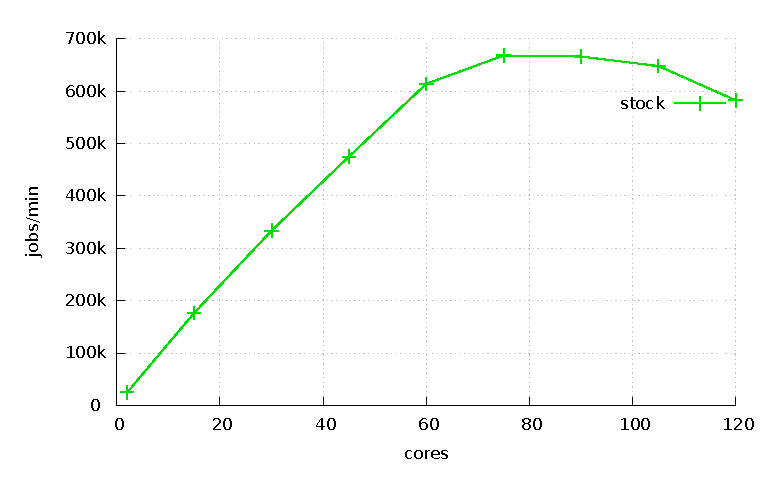
\includegraphics[scale=0.65]{graph/aim7_default.eps}
%  \end{center}
%  \caption{Scalability of AIM7 multiuser. This workload simultaneously create
%  many processes.
%  Up to 60 core, the stock Linux scale linearly, then they flattens out.}
%  \label{fig:aim7_default}
%\end{figure}
 
%In this section, we describe how to apply our concurrent update based on
%deferred update method to Linux.
%The Linux fork is associate with an anonymous page and a file page.
%When many processes are simultaneously created in Linux, 
%these two reverse mapping
%can become bottlenecks since their data structures are shared between
%processes.
%Figure~\ref{fig:aim7_default} shows the scalability problem in case
%of the fork-intensive workload that simultaneously creates many processes.
%Up to 60 core, the stock Linux scales linearly, then creating the reverse
%mapping becomes the bottleneck because their interval trees are protected by
%locks.
%Therefore, fork-intensive workload can pose a scalability bottleneck due to the
%update-heavy data
%structures~\cite{SilasBoydWickizerPth}~\cite{Andi2011adding}~\cite{Tim2013adding}.

%Figure mapped page에 대에 적용한  그림
%\begin{figure}[tb]
%%  \begin{center}
    %
    % \includegraphics[width=0.5\textwidth,height=0.5\textheight,keepaspectratio]{fig/deferu}
%  \end{center}
%  \caption{An example of applying the \deferu to file reverse mapping. }
%  \label{fig:deferu}
%\end{figure}


%Paragraph 6: DeferU 알고리즘 적용 - Mapped page - 리눅스 자료구조를 수정
%Figure~\ref{fig:deferu} gives an example of applying the \deferu to file
%reverse mapping and shows relationship between interval trees and lock-less
% lists.
%An interval tree contains two \code{virtual memory area}(\code{VMA}) nodes; 
%on the other hand, the lock-less list contains the right \code{VMA} as shown in
%Figure~\ref{fig:deferu}.
%It means that the right \code{VMA} has been deleted, and the synchronization
% has not been invoked. 

%In order to using the \deferu, the data structures involved in the
%head(\code{address\_space}) or the node(\code{vm\_area\_structure}) can be
% modified with \deferu's structure as shown in Figure~\ref{fig:deferu}. 
%In addition, programmer must replace \emph{physical update} with \emph{logical
%update} to eliminate the lock. 
%Before the corresponding readers need to be read, \deferu must call synchronize
%function to keep the consistency.
